\chapter{Kvante-logiske porter}

Beregninger i en klassisk datamaskin blir gjort av logiske porter som tar inn en eller flere bit og gir ut en eller flere bit som svar. For eksempel tar en AND-port inn to bit og gir ut svaret 1 dersom begge inn-bitene er 1, ellers gir den ut svaret 0. Tilsvarende blir beregninger i en kvantedatamaskin gjort av kvante-logiske porter som tar inn en eller flere qubit og gir ut en eller flere qubit som svar. Likhetene mellom de to typer datamaskiner er altså store, men vi skal etter hvert se at kombinasjonen av at en qubit kan være i en superposisjon mellom 0 og 1 og at to eller flere qubit kan være sammenfiltret gir kvantedatamaskinen muligheter som går langt utover det klassiske datamaskiner har.

\section{Logiske porter og boolsk algebra}
På grunn av den klare analogien med vanlige logiske porter er det nyttig å ha dette friskt i minne når vi skal studere kvante-logiske porter. Derfor gir jeg et kort overblikk av klassiske logiske porter og hvordan de kan kombineres før jeg introduserer den kvantemekaniske versjonen. 

\subsection{Boolsk algebra}
Matematikken som brukes for å analysere logiske porter\footnote{Ofte brukes begrepet operasjoner i stedet for porter, spesielt når man snakker om boolsk algebra på et mer abstrakt nivå. Det er et en-til-en forhold mellom operasjonene i boolsk algebra og logiske porter anvendt i logiske kretser så distinksjonen mellom operasjoner og porter er ikke viktig.} og nettverk av slike er boolsk algebra. Boolsk algebra er en enkel algebra som opererer på variabler som kun kan ha to mulig verdier: SANT eller USANT. I en datamaskin assosieres SANT med bit-verdien 1 og USANT med bit-verdien 0, og i det videre vil jeg bruke 1 og 0 som de mulige verdiene til de boolske variablene. De grunnleggende regneoperasjonene i den boolske algebraen er:

\subsubsection{NOT (symbol $\neg$)}
NOT er en port/operasjon som tar inn en bit og gir ut en bit. En NOT-port vil alltid endre bit-verdien til det motsatte som vist i sannhetstabellen nedenfor.
\begin{center}
\begin{figure}[h]
\begin{subfigure}{.3\textwidth}
	\begin{tabular}{|c|c|}
	\hline
	$P$ & $\neg P$ \\
	\hline
	0 & 1 \\
	1 & 0 \\
	\hline
	\end{tabular}
\end{subfigure}
\begin{subfigure}{.3\textwidth}
	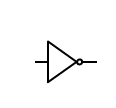
\includegraphics{./gate_not}
\end{subfigure}
\caption{Venstre: Sannhetstabell for NOT-operatoren. Høyre: Kretssymbol for NOT-port.}
\end{figure}
\end{center}

\subsubsection{AND (symbol $\land$)}
AND er en port/operasjon som tar inn to bit og gir ut en bit. AND gir ut 1 dersom begge inn-bitene er 1, ellers gir den ut 0 som vist i sannhetstabellen nedenfor.
\begin{center}
\begin{figure}[h]
\begin{subfigure}{.3\textwidth}
	\begin{tabular}{|c|c|c|}
	\hline
	$P$ & $Q$ & $P \land Q$ \\
	\hline
	0 & 0 & 0\\
	0 & 1 & 0 \\
	1 & 0 & 0 \\
	1 & 1 & 1 \\
	\hline
	\end{tabular}
\end{subfigure}
\begin{subfigure}{.3\textwidth}
	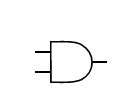
\includegraphics{./gate_and}
\end{subfigure}
\caption{Venstre: Sannhetstabell for AND-operatoren. Høyre: Kretssymbol for AND-port.}
\end{figure}
\end{center}

\subsubsection{OR (symbol $\lor$)}
OR er en port/operasjon som tar inn to bit og gir ut en bit. OR gir ut 1 dersom minst \'en av inn-bitene er 1, ellers gir den ut 0 som vist i sannhetstabellen nedenfor.
\begin{center}
\begin{figure}[h]
\begin{subfigure}{.3\textwidth}
	\begin{tabular}{|c|c|c|}
	\hline
	$P$ & $Q$ & $P \lor Q$ \\
	\hline
	0 & 0 & 0\\
	0 & 1 & 1 \\
	1 & 0 & 1 \\
	1 & 1 & 1 \\
	\hline
	\end{tabular}
\end{subfigure}
\begin{subfigure}{.3\textwidth}
	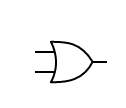
\includegraphics{./gate_or}
\end{subfigure}
\caption{Venstre: Sannhetstabell for OR-operatoren. Høyre: Kretssymbol for OR-port.}
\end{figure}
\end{center}

\subsection{Sammensatte porter}
De ulike portene som er presentert ovenfor kan kombineres til å representere en vilkårlig bineær funksjon\footnote{Det kan vises at det er tilstrekkelig med operasjonene $\neg$ og $\land$ for å oppnå dette, men det er likvel en vanlig konvensjon å beholde $\lor$ på listen over de grunnleggende logiske operasjonene.}, altså en funksjon som tar et antall bit inn og gir ut et antall bit ut med en spesifisert regel for hva som ut verdien(e) blir gitt innverdien(e). Noen slike kombinasjoner er spesielt hyppig brukt og har derfor fått egne navn og symboler. Dette inkluderer:

\subsubsection{XOR (symbol $\oplus$)}
XOR, eller exclucive or, er en operasjon/port som tar inn to bit og gir ut en bit. Denne representerer en enten/eller, altså en port som gir ut verdien 1 hvis \'en, men ikke begge inn-bitene har verdien 1. Ellers gir den ut verdien 0. XOR kan konstrueres som $P\oplus Q = (P\land\neg Q)\lor(\neg P \land Q)$. 
\begin{center}
\begin{figure}[h]
\begin{subfigure}{.3\textwidth}
	\begin{tabular}{|c|c|c|}
	\hline
	$P$ & $Q$ & $P \oplus Q$ \\
	\hline
	0 & 0 & 0\\
	0 & 1 & 1 \\
	1 & 0 & 1 \\
	1 & 1 & 0 \\
	\hline
	\end{tabular}
\end{subfigure}
\begin{subfigure}{.3\textwidth}
	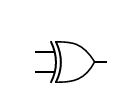
\includegraphics{./gate_xor}
\end{subfigure}
\caption{Venstre: Sannhetstabell for XOR-operatoren. Høyre: Kretssymbol for XOR-port.}
\end{figure}
\end{center}

\subsubsection{NAND (symbol $\uparrow$)}
NAND er en kombinasjon av NOT og AND. Den tar inn to bit og gir ut en bit. Siden NOT er kombinert med AND gir den alltid ut den motsatte verdien av hva AND ville gjort. NAND kan konstrueres som $P \uparrow Q = \neg(P\land Q)$. 

\begin{center}
\begin{figure}[h]
\begin{subfigure}{.3\textwidth}
	\begin{tabular}{|c|c|c|}
	\hline
	$P$ & $Q$ & $P \oplus Q$ \\
	\hline
	0 & 0 & 1\\
	0 & 1 & 1 \\
	1 & 0 & 1 \\
	1 & 1 & 0 \\
	\hline
	\end{tabular}
\end{subfigure}
\begin{subfigure}{.3\textwidth}
	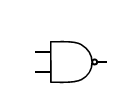
\includegraphics{./gate_nand}
\end{subfigure}
\caption{Venstre: Sannhetstabell for NAND-operatoren. Høyre: Kretssymbol for NAND-port.}
\end{figure}
\end{center}

\section{Generalisering til kvante-logiske porter}
For å lage en kvantedatamaskin trenger vi å lage en qubit-versjon av portene som er diskutert ovenfor. Vi støter da straks på en interessant utfordring: mens en klassisk bit alltid er enten 0 eller 1 vil en qubit generelt være i en superposisjon av 0 og 1. Hvordan skal vi lage sannhetstabellene når qubitene har et kontinuerlig sett av mulige verdier? La oss først få på plass litt notasjon som er nyttig i den videre diskusjonen. Nå er det tilstrekkelig for oss å jobbe med \'en basis, og der velger vi $\left\{ \left[\begin{array}{cc}1\\0\end{array}\right], \left[\begin{array}{cc}1\\0\end{array}\right] \right\}$. For å forenkle notasjonen litt kommer jeg for det meste til å skrive vektorene i bra-ket notasjon, med der basisvektorene er identifisert som
\begin{displaymath}
	|0\rangle = \left[\begin{array}{cc}1\\0\end{array}\right] \text{ og } |1\rangle =  \left[\begin{array}{cc}1\\0\end{array}\right].
\end{displaymath}
En generell qubit kan da skrives som $|a\rangle = a_0|0\rangle + a_1|1\rangle$ der $a_0^2 + a_1^2 = 1$. Når vi måler verdien av denne qubiten vil vi finne enten $|0\rangle$ eller $|1\rangle$ med sannynligheter henholdsvis $a_0^2$ og $a_1^2$. Hvis vi har mer enn en qubit å ta hensyn til, må vi ta tensorproduktet av basisvektorene for å finne den nye basisen. For eksempel er basisen for to qubit
\begin{displaymath}
	\left\{ |0\rangle\otimes|0\rangle,  |0\rangle\otimes|1\rangle,  |1\rangle\otimes|0\rangle,  |1\rangle\otimes|1\rangle  \right\}.
\end{displaymath}
For å forenkle notasjonen ytterligere innfører vi konvensjonen at $|00\rangle = |0\rangle\otimes|0\rangle$ og så videre, slik at basisen kan skrives som
\begin{displaymath}
	\left\{ |00\rangle,  |01\rangle,  |10\rangle,  |11\rangle  \right\}.
\end{displaymath}
En generell kombinasjon av to qubit kan da skrives som $|b\rangle = b_{00}|00\rangle + b_{01}|01\rangle + b_{10}|10\rangle + b_{11}|11\rangle$ der $b_{00}^2 + b_{01}^2 + b_{10}^2 + b_{11}^2 = 1$. 

\subsection{Ingen kloning-teoremet}
Vi treffer på en annen viktig forskjell mellom klassisk logikk og kvantelogikk dersom vi ønsker å klone en qubit---det vil si å lage en ekstra kopi av en qubit som er identisk med den vi har. Med klassiske bit er dette ikke noe problem. Hvis vi har en bit med en vilkårlig verdi kan vi uten problemer lage vilkårlig mange kopier av denne. Slik er det ikke i kvanteverden. Det kan vises at i det generelle tilfellet kan man ikke lage en kopi av en qubit slik at man sitter igjen med to qubit som er identiske og lik den vi startet med. Så lenge vi jobber med qubit som har en bestemt verdi er det riktignok ingen forskjell, men for å utnytte oss av fordelene som kan oppnås ved å bruke qubit i superposisjon mellom ulike verdier må algoritmene i en kvantedatamaskin lages på en slik måte at kloning av qubit er unødvendig.

Jeg vil ikke forsøke å bevise ingen kloning-teoremet her, men kun gi kvalitative argumenter som sannsynliggjør at det er riktig. En vilkårlig qubit kan som tidligere beskrevet skrives som $|a\rangle = a_0|0\rangle + a_1|1\rangle$. Dersom vi ønsker å måle verdien av qubiten vil vi aldri få noe annet enn $|0\rangle$ eller $|1\rangle$. Hvis vi kjenner $a_0$ og $a_1$ kan vi riktignok beregne sannsynligheten for hvert av de to ulike måleresultatene, men hva hvis vi har en qubit i en ukjent tilstand? Dersom vi for eksempel får resultatet $|0\rangle$ er det eneste vi kan si om koeffisientene at $a_0>0$. Vi kan altså ikke måle oss frem til hva koeffisientene $a_0$ og$a_1$ er. Men hvis vi ikke kan hente ut denne informasjonen, hvordan kan vi da lage en identisk kopi? 